\documentclass{article}
    \usepackage{amssymb}
    \usepackage[utf8]{inputenc}
    \usepackage[russian]{babel}
    \usepackage[left=2cm,right=2cm,
        top=2cm,bottom=2cm,bindingoffset=0cm]{geometry}
    \usepackage{hyperref}
    \hypersetup{
        colorlinks=true,
        linkcolor=blue,
        filecolor=magenta,      
        urlcolor=cyan,
    }
  \usepackage{graphicx}
  \usepackage{booktabs}
  \graphicspath{{pictures/}}
  \DeclareGraphicsExtensions{.pdf,.png,.jpg}
\usepackage{subcaption}
%\captionsetup{compatibility=false}

\begin{document}
\begin{center}{\hugeОтчет по курсовой работе за неделю\\}\end{center}
Дата: 25.2.2021\\
Научные руководители: Герасимов С.В., Мещеряков А.В.\\
Студент: Немешаева Алиса\\
Курс: 4\\

\renewcommand{\labelitemi}{$\blacksquare$}
\renewcommand\labelitemii{$\square$}
\begin{enumerate}
    \item Построена кривая обучения для модели act\_found2.\\
    \item Построена таблица откликов для скоплений с разными параметрами M500 и z (промежутки для 
        M500 и z были выбраны так, чтобы в каждой группе оказалось равное по сравнению с остальными
        количество объектов). Результаты представлены в таблице ~\ref{Tab:Tcr}{}.\\
    \item Исправлена иллюстрация для демонстрации карты сегментации модели all\_found34. 
        ~\ref{Pic:Cluster}{}\\
\end{enumerate}



\begin{table}
\begin{tabular}{lrrrrrr}
\toprule
{} &  (0.00,0.15) &  (0.15,0.28) &  (0.28,0.41) &  (0.41,0.55) &  (0.55,0.72) &  (0.72,2.00) \\
\midrule
0 &     0.029412 &     0.038835 &     0.048544 &     0.049020 &     0.038835 &     0.039216 \\
1 &     0.019417 &     0.147059 &     0.137255 &     0.088235 &     0.029412 &     0.029126 \\
2 &     0.088235 &     0.205882 &     0.088235 &     0.049505 &     0.049020 &     0.019608 \\
3 &     0.254902 &     0.176471 &     0.107843 &     0.106796 &     0.058252 &     0.049020 \\
4 &     0.411765 &     0.267327 &     0.178218 &     0.107843 &     0.049020 &     0.039216 \\
5 &     0.558824 &     0.384615 &     0.221154 &     0.156863 &     0.049020 &     0.039216 \\
6 &     0.627451 &     0.745098 &     0.401961 &     0.215686 &     0.089109 &     0.087379 \\
7 &     0.754902 &     0.862745 &     0.715686 &     0.274510 &     0.086538 &     0.088235 \\
8 &     0.813725 &     0.862745 &     0.970588 &     0.529412 &     0.215686 &     0.127451 \\
9 &     0.873786 &     0.980583 &     0.961165 &     0.932039 &     0.737864 &     0.359223 \\
\bottomrule
\end{tabular}
\caption{Результаты отклика для различных диапазонов M500 и z для каталога pz\_rot\_28.}
\label{Tab:Tcr}
\end{table}

\begin{figure}[h]
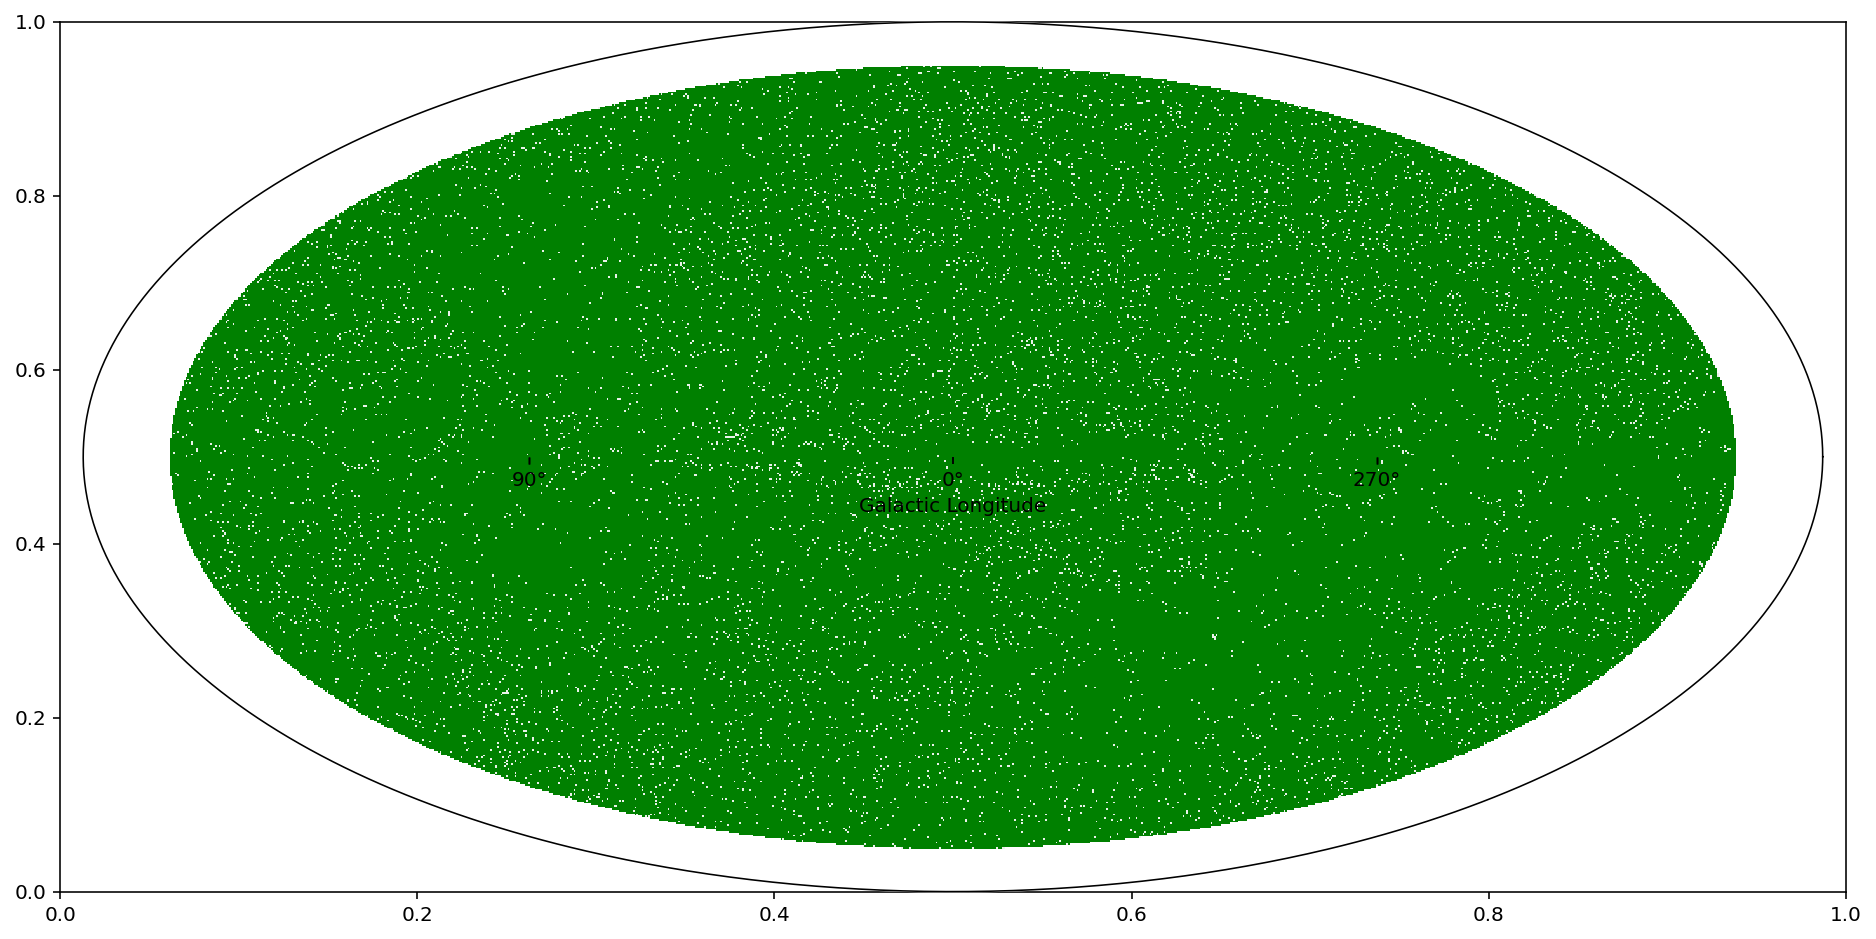
\includegraphics[width=0.8\linewidth]{pz_rot28_map}
\caption{Распределение найденных моделью pz\_rot28 скоплений по небу}
\end{figure}

\begin{figure}[h]
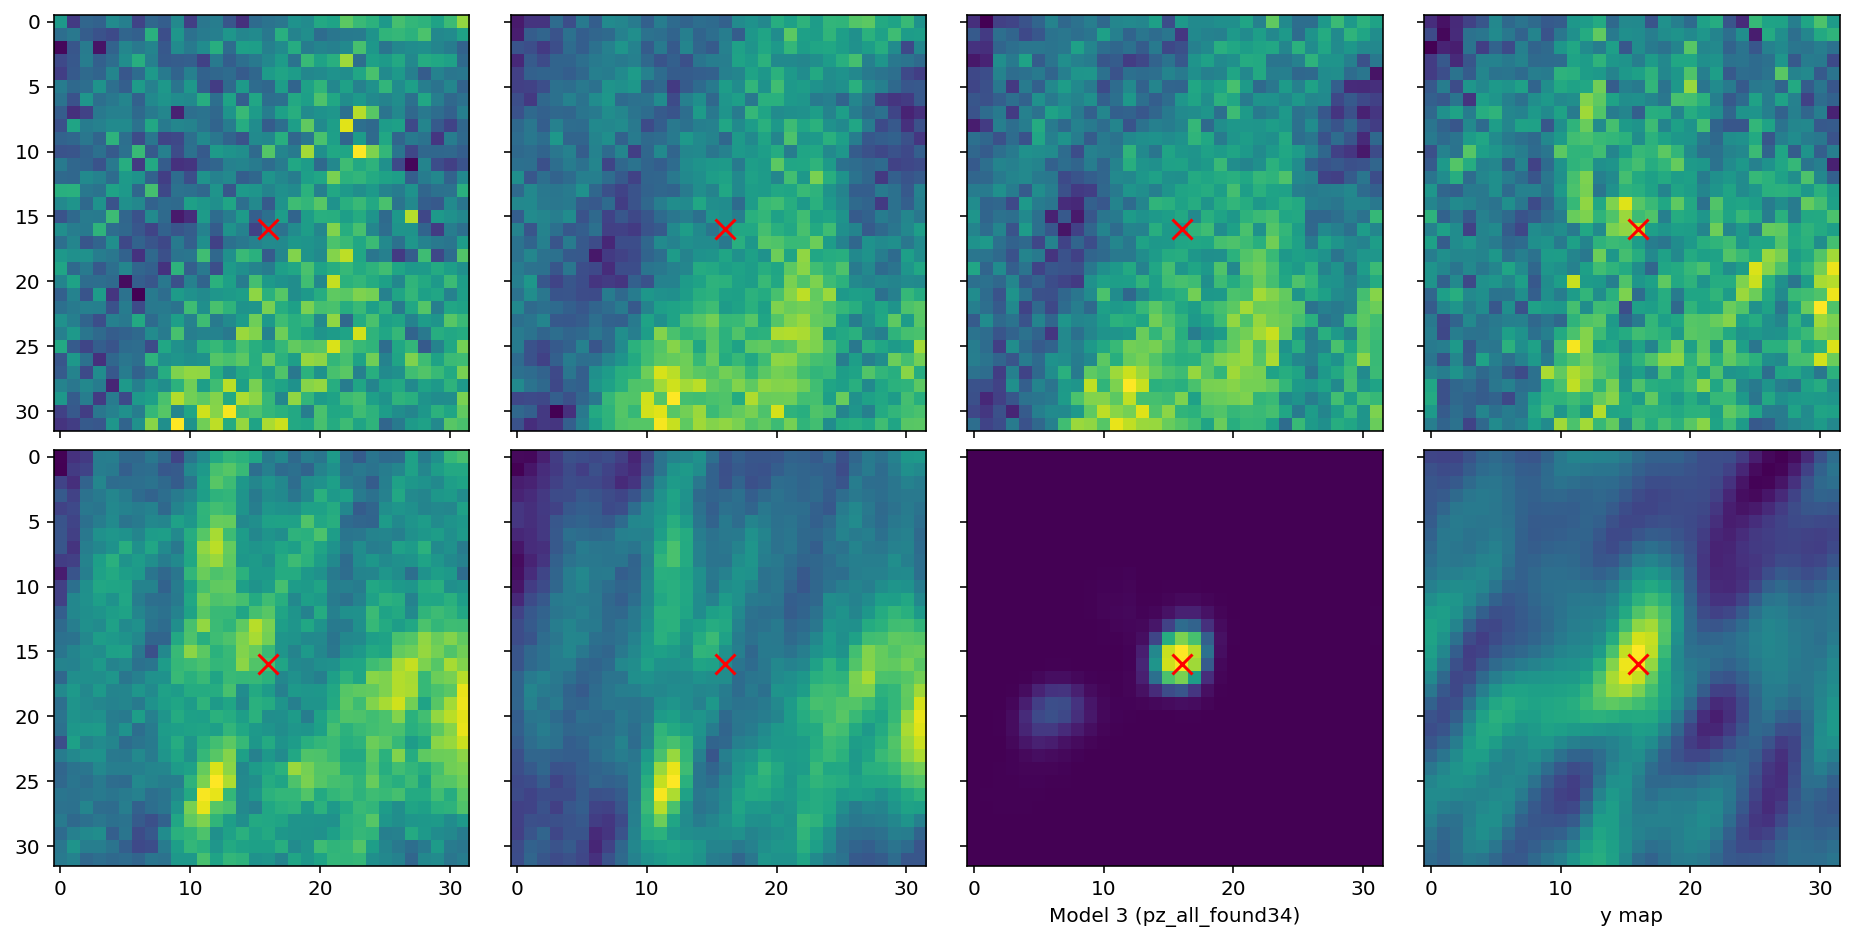
\includegraphics[width=0.8\linewidth]{cluster_pic}
\caption{Скопление из каталога planck\_z (RA 166.422, DEC -10.2505) с картами Planck, картой 
    сегментации и картой y-параметра.}
\label{Pic:Cluster}
\end{figure}

Отчет согласован с научным руководителем.\\
Общее количество строк кода за эту неделю: 218\\
\href{https://github.com/rt2122/data-segmentation-2}{Репозиторий}\\ 
\end{document}
